\documentclass[10pt,handout]{beamer}

\usetheme{metropolis}
\usepackage{appendixnumberbeamer}

\usepackage[spanish]{babel}
\usepackage[utf8]{inputenc}

\usepackage{booktabs}
\usepackage[scale=2]{ccicons}

\usepackage{tikz}
\usetikzlibrary{matrix}

\usepackage{pgfplots}
\usepgfplotslibrary{dateplot}


\usepackage{xspace}
\usepackage{epsfig}
\usepackage{color}
\usepackage{listings}
\usepackage[]{algorithm2e}
\usepackage{tikz}
\newcommand{\themename}{\textbf{\textsc{metropolis}}\xspace}
\graphicspath{{./data/}{./resources/}}
\definecolor{mygray}{gray}{0.4}

\usepackage[normalem]{ulem}

\title{Taller de programación competitiva}
\subtitle{\textit{An amateur approach}}
\date{20 de febrero de 2018}
\author{
  Ignacio Ballesteros González\\
  {\color{mygray}\texttt{ballesteros@acm.org}\\}
  \\
  Samuel García Haro\\
  {\color{mygray}\texttt{samgh96@gmail.com}\\}
}

\institute{}
\titlegraphic{\hfill
\includegraphics[height=1.5cm]{acm_png.png}}

\begin{document}

\maketitle

\begin{frame}{¿Quiénes somos y por qué queremos hacer esto?}
  \begin{columns}[onlytextwidth]
    \begin{column}{0.3\textwidth}
      \centering
      \begin{itemize}
      \item Somos presidente y vicepresidente del capítulo de ACM.
      \item Somos veteranos en ser vapuleados en competiciones.
      \item Experiencia instructiva y cura de humildad.
      \end{itemize}
    \end{column}
    \begin{column}{0.3\textwidth}
      \centering
      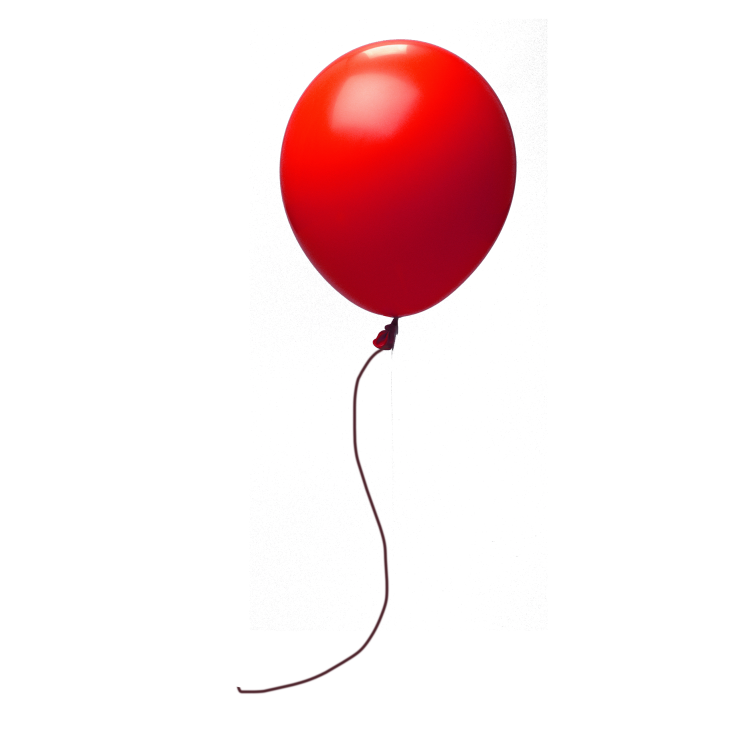
\includegraphics[width=\textwidth]{globo.png}
    \end{column}
    \begin{column}{0.35\textwidth}
      En cuanto a informática:
      \begin{itemize}
      \item No nos dedicamos a esto.
      \item No nos gusta Java.
      \item Nos gusta funcional.
      \end{itemize}
    \end{column}
  \end{columns}
\end{frame}

\begin{frame}{Índice}
  \setbeamertemplate{section in toc}[sections numbered]
  % \setbeamertemplate{subsection in toc}[subsections numbered]
  \tableofcontents%[hideallsubsections]
\end{frame}

\section{Introducción}

\begin{frame}{Algunos recursos}
  \texttt{Comptetitive Programming 3 - Steve Halim, Felix Halim}
  \texttt{https://cpbook.net/}
  \emph{(Próximamente en la biblioteca de ACM)}
  \begin{center}
    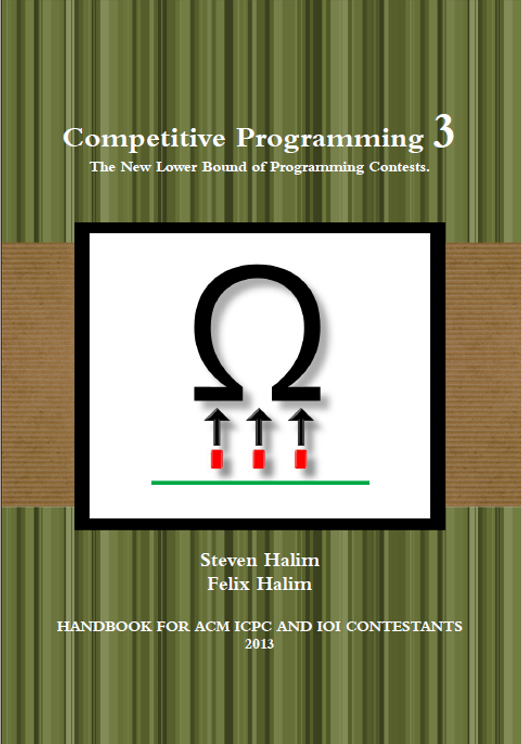
\includegraphics[height=5cm]{cp3.png}
  \end{center}
  \texttt{https://www.geeksforgeeks.org/}
\end{frame}

\section{Estructuras de datos}

\begin{frame}{El papel de las estructuras de datos}
  Una buena estructura de datos nos facilita la modelización del problema.
  \begin{itemize}
  \item Son el campo de juego de nuestros algoritmos.
  \item Conocer el lenguaje y sus librerías nos ahorra mucho trabajo.
  \end{itemize}
  Sin embargo, este ahorro no nos exime de la responsabilidad.
  \begin{itemize}
  \item Debemos saber la complejidad de las estructuras.
  \item Debemos identificar cuáles son mejores para cada caso.
  \item Debemos conocer sus puntos fuertes y débiles.
  \end{itemize}
\end{frame}

\begin{frame}{Estructuras de datos lineales}
  Array estático:
  \begin{itemize}
  \item Soportado nativamente.
  \item La estructura básica más utilizada.
  \end{itemize}
  Array dinámico:
  \begin{itemize}
  \item Cambiamos su tamaño en tiempo de ejecución.
  \item \texttt{ArrayList} o \texttt{Vector}
  \end{itemize}
  Podemos usar algoritmos como \texttt{sort} o \texttt{binarySearch}
  sobre las estructuras. (Librerías: \texttt{Arrays},
  \texttt{Collections})
\end{frame}

\begin{frame}{Estructuras de datos lineales}
  \begin{columns}
    \begin{column}{0.5\textwidth}
      Pilas:
      \begin{itemize}
      \item Last Input First Output (LIFO)
      \item \texttt{Java Stack}
      \end{itemize}

      \vspace{20pt}

      \centering\begin{tikzpicture}[draw, minimum width=1cm, minimum height=0.5cm]
        \node[draw] (in) at (-1,2) {};
        \node[draw] (out) at (1,2) {};
        \matrix (queue)[matrix of nodes, nodes={draw, nodes={draw}}, nodes in empty cells]
        {
          ~~~~\\~~~~\\ \\ \\
        };

        \draw[-latex] (0.25,1) .. controls (0.25,1.5) and (1,1.5)  .. node[below right] {\small pop()} (out.south);
        \draw[-latex] (in.south) .. controls (-1, 1.5) and (-0.25,1.5) .. node[below left] {\small push()} (-0.25,1);
      \end{tikzpicture}
    \end{column}
    \begin{column}{0.5\textwidth}
      Colas:
      \begin{itemize}
      \item First Input First Output (FIFO)
      \item \texttt{Java Queue}
      \end{itemize}

      \centering\begin{tikzpicture}[draw, minimum width=1cm, minimum height=0.5cm]
        \node[draw] (in) at (-1,2) {};
        \node[draw] (out) at (1,-2) {};
        \matrix (queue)[matrix of nodes, nodes={draw, nodes={draw}}, nodes in empty cells]
        {
          \\ \\ \\ \\
        };

        \draw[-latex] (0.25,-1) .. controls (0.25,-1.25) and (1,-1.25) .. node[below left] {\small pop()} (out.north);
        \draw[-latex] (in.south) .. controls (-1, 1.5) and (-0.25,1.5) .. node[below left] {\small push()} (-0.25,1);
      \end{tikzpicture}

      \vspace{-10pt}
    \end{column}
  \end{columns}
\end{frame}

\begin{frame}{Estructuras de datos no lineales}
  Árboles binarios de búsqueda:
  \begin{itemize}
  \item El subárbol izquierdo de un nodo contiene valores menores.
  \item El subárbol derecho de un nodo contiene valores mayores.
  \end{itemize}
  \centering 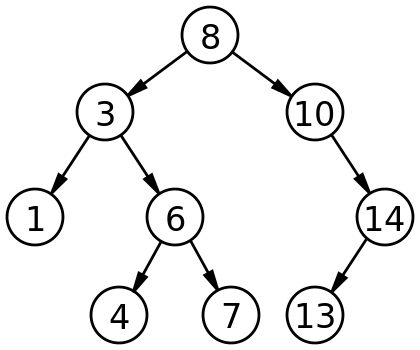
\includegraphics[height=4cm]{bst.png}

  \texttt{Java TreeMap} $(clave \implies valor)$

  \texttt{Java TreeSet} $(clave)$
\end{frame}

\begin{frame}{Otras estructuras de datos}
  \begin{itemize}
  \item Colas con priodidad (\emph{Heap})
  \item Grafos
    \begin{itemize}
    \item Matriz de adyacencia
    \item Lista de nodos adyacentes
    \item Lista de aristas
    \end{itemize}
  \item Más árboles.
  \item ...
  \end{itemize}
\end{frame}

\section{Entrada/Salida}
\begin{frame}{Entrada/Salida}
  \begin{itemize}
  \item La entrada nos da pistas de la modelización del problema. \pause
  \item Es importante \textbf{no perder más tiempo del necesario con la E/S}. \pause
  \item Se recomienda llevarla apuntada o en su defecto memorizarla.
  \end{itemize}
\end{frame}


\begin{frame}{Entrada/Salida: Entrada}
  \texttt{4 -> número de entradas \newline \pause
    4 -> tamaño de vector \newline \pause
    1 1 1 2 -> elementos de vector \newline \pause
    2 \newline
    1 1 \newline
    5 \newline
    1 1 2 2 3 \newline
  }
\end{frame}

\begin{frame}{Entrada/Salida: Procesador genérico}
  \begin{algorithm}[H]
    \KwData{num\_entradas, tam\_vector, vector}
    declarar variables\;
    \While{num\_entradas \textgreater 0}{
      leer tam\;
      inicializar vector\;
      \For{$i$ in \KwTo tam\_vector}{
        vector[i] = leer\_entero\;
      }
      procesar\;
      num\_entradas -= 1\;
    }
  \end{algorithm}
\end{frame}
\defverbatim[colored]\lstES{
  \begin{lstlisting}[language=Java,basicstyle=\ttfamily,keywordstyle=\color{blue}]
    public static void main(String[] args){
      int n, len;
      int [] arr;
      FastReader fr = new FastReader();

      n = fr.nextInt();
      while (n > 0){
        len = fr.nextInt();
        arr = new int[len];
        for (int i = 0; i < len; i++)
        arr[i] = fr.nextInt();

        System.out.println(findMajority(arr));
        n--;
      }
    }
  \end{lstlisting}
}

\begin{frame}{Entrada/Salida: Ejemplo}
  \lstES
\end{frame}
\section{Métodos algorítmicos}

\subsection{Divide y vencerás}
\begin{frame}{Divide y vencerás: Concepto}
  \begin{itemize}
  \item Patrón de diseño de algoritmos de carácter recursivo. \pause
  \item Descompone problemas en subproblemas de solución más sencilla. \pause
  \item Se distinguen cuatro pasos: \pause
    \begin{itemize}
    \item Hallar el caso base del problema. \pause
    \item Dividir la estructura de datos hasta encontrar el caso base. \pause
    \item Aplicar la solución al caso base. \pause
    \item Recomponer la estructura de datos ya resuelta. \pause
    \end{itemize}
  \item Ejemplos de este método: Mergesort, quicksort, búsqueda binaria...
  \end{itemize}
\end{frame}
\begin{frame}{Divide y vencerás: Árbol de recursión}
  \centering
  \begin{tikzpicture}[level/.style={sibling distance=12mm}]
    \node [draw] (z){n}
    child [grow=right] {node (w) {} edge from parent[draw=none]
      child [grow=right] {node (x) {Estructura de entrada} edge from parent[draw=none]
      }
    }
    child {node [draw] (a) {$\frac{n}{2}$}
      child {node [draw] (b) {$\frac{n}{2^2}$}
        child {node {$\vdots$}
          child {node [draw] (d) {$\frac{n}{2^k}$}}
          child {node [draw] (e) {$\frac{n}{2^k}$}}
        }
        child {node {$\vdots$}}
      }
      child {node [draw] (g) {$\frac{n}{2^2}$}
        child {node {$\vdots$}}
        child {node {$\vdots$}}
      }
    }
    child {node [draw] (j) {$\frac{n}{2}$}
      child {node [draw] (k) {$\frac{n}{2^2}$}
        child {node {$\vdots$}}
        child {node {$\vdots$}}
      }
      child {node [draw] (l) {$\frac{n}{2^2}$}
        child {node {$\vdots$}}
        child {node (c){$\vdots$}
          child {node [draw] (o) {$\frac{n}{2^k}$}}
          child {node [draw] (p) {$\frac{n}{2^k}$}
            child [grow=right] {node (q) {$=>$} edge from parent[draw=none]
              child [grow=right] {node (q) {Caso base} edge from parent[draw=none]
              }
            }
          }
        }
      }
    };
  \end{tikzpicture}
\end{frame}
\subsection{Método voraz}
\begin{frame}{Método voraz: Concepto}
  \begin{itemize}
  \item Este método algorítmico se basa en la elección de soluciones locales óptimas
    con el fin de obtener soluciones globales óptimas. \pause
  \item Útil en problemas de optimización pero difícil de probar su correctitud. \pause
  \item Consiste en los siguientes fundamentos: \pause
    \begin{itemize}
    \item Disponemos de un conjunto de entrada (candidatos) y de otro de salida. \pause
    \item Mediante heurísticas decidimos qué elemento entra en el conjunto de salida
      (y lo eliminamos de los candidatos). \pause
    \item Para decidir los siguientes elementos los sometemos a un test de factibilidad. \pause
    \end{itemize}
  \item Ejemplos: A*, Prim, Kruskal, TSP...
  \end{itemize}
\end{frame}
\pgfdeclarelayer{background}
\pgfsetlayers{background,main}

\begin{frame}{Método voraz: Diagrama de ejemplo (Prim)}

%% Adjacency matrix of graph
%% \  a  b  c  d  e  f  g
%% a  x  7     5
%% b  7  x  8  9  7
%% c     8  x     5
%% d  5  9     x 15  6
%% e     7  5 15  x  8  9
%% f           6  8  x 11
%% g              9  11 x

\tikzstyle{vertex}=[circle,fill=black!25,minimum size=20pt,inner sep=0pt]
\tikzstyle{selected vertex} = [vertex, fill=red!24]
\tikzstyle{edge} = [draw,thick,-]
\tikzstyle{weight} = [font=\small]
\tikzstyle{selected edge} = [draw,line width=5pt,-,red!50]
\tikzstyle{ignored edge} = [draw,line width=5pt,-,black!20]

\begin{figure}
\begin{tikzpicture}[scale=1.8, auto,swap]
    % Draw a 7,11 network
    % First we draw the vertices
    \foreach \pos/\name in {{(0,2)/a}, {(2,1)/b}, {(4,1)/c},
                            {(0,0)/d}, {(3,0)/e}, {(2,-1)/f}, {(4,-1)/g}}
        \node[vertex] (\name) at \pos {$\name$};
    % Connect vertices with edges and draw weights
    \foreach \source/ \dest /\weight in {b/a/7, c/b/8,d/a/5,d/b/9,
                                         e/b/7, e/c/5,e/d/15,
                                         f/d/6,f/e/8,
                                         g/e/9,g/f/11}
        \path[edge] (\source) -- node[weight] {$\weight$} (\dest);
    % Start animating the vertex and edge selection. 
    \foreach \vertex / \fr in {d/1,a/2,f/3,b/4,e/5,c/6,g/7}
        \path<\fr-> node[selected vertex] at (\vertex) {$\vertex$};
    % For convenience we use a background layer to highlight edges
    % This way we don't have to worry about the highlighting covering
    % weight labels. 
    \begin{pgfonlayer}{background}
        \pause
        \foreach \source / \dest in {d/a,d/f,a/b,b/e,e/c,e/g}
            \path<+->[selected edge] (\source.center) -- (\dest.center);
        \foreach \source / \dest / \fr in {d/b/4,d/e/5,e/f/5,b/c/6,f/g/7}
            \path<\fr->[ignored edge] (\source.center) -- (\dest.center);
    \end{pgfonlayer}
\end{tikzpicture}
\end{figure}

\end{frame}
\subsection{Programación dinámica}


\begin{frame}{Programacion Dinámica}

  Saber resolver problemas con Programación Dinámica es clave para la
  programación competitiva.

  \begin{itemize}
  \item Hay veces que la resolución mediante \emph{Divide y vencerás}
    lleva a la repetición de casos ya estudiados. Este problema
    incrementa la complejidad del algoritmo.

  \item La \textbf{base} de la programación dinámica es el uso de una
    \textbf{tabla} para ir almacenando los resultados que puedan
    usarse posteriormente.

  \item La programación dinámica normalmente se usa para resolver
    problemas de \emph{Optimización} y problemas de \emph{Conteo}.

  \end{itemize}
\end{frame}
\end{document}